\chapter{Bioinorganic Chemistry}\label{ch:b3:bioinorganic}

Our blood is red because of iron; the blood of a horseshoe crab is colourless in
its veins and turns blue in air, because it carries oxygen on copper. Life uses
a handful of metal ions for the jobs no organic group can do: binding oxygen
reversibly, moving single electrons, splitting water, reducing nitrogen,
making a water molecule acidic enough to attack carbon dioxide. This chapter
reads those jobs with the tools of coordination chemistry: hard and \omterm{def:b3:bioinorganic:hsab}{soft
acids}, ligand fields and spin states, equilibria and rate laws, and it ends
with the metals used as drugs.

\begin{recall}
The Year 2 volume treated $\alpha$-amino acids, side chains and peptides, nucleobases
and nucleotides, coordination complexes, ligand fields, high and low spin, and
hard and soft nucleophiles and electrophiles; the Year 1 volume complexation
constants and the pL scale. \Cref{ch:b3:complex-spectra-magnetism} and
\cref{ch:b3:complex-mechanisms} gave spectra, Marcus theory and the aquation of
cisplatin, \cref{ch:b3:complex-kinetics} Michaelis--Menten kinetics, and
\cref{ch:b3:advanced-nmr} the relaxation time $T_1$.
\end{recall}

\begin{omfigure}
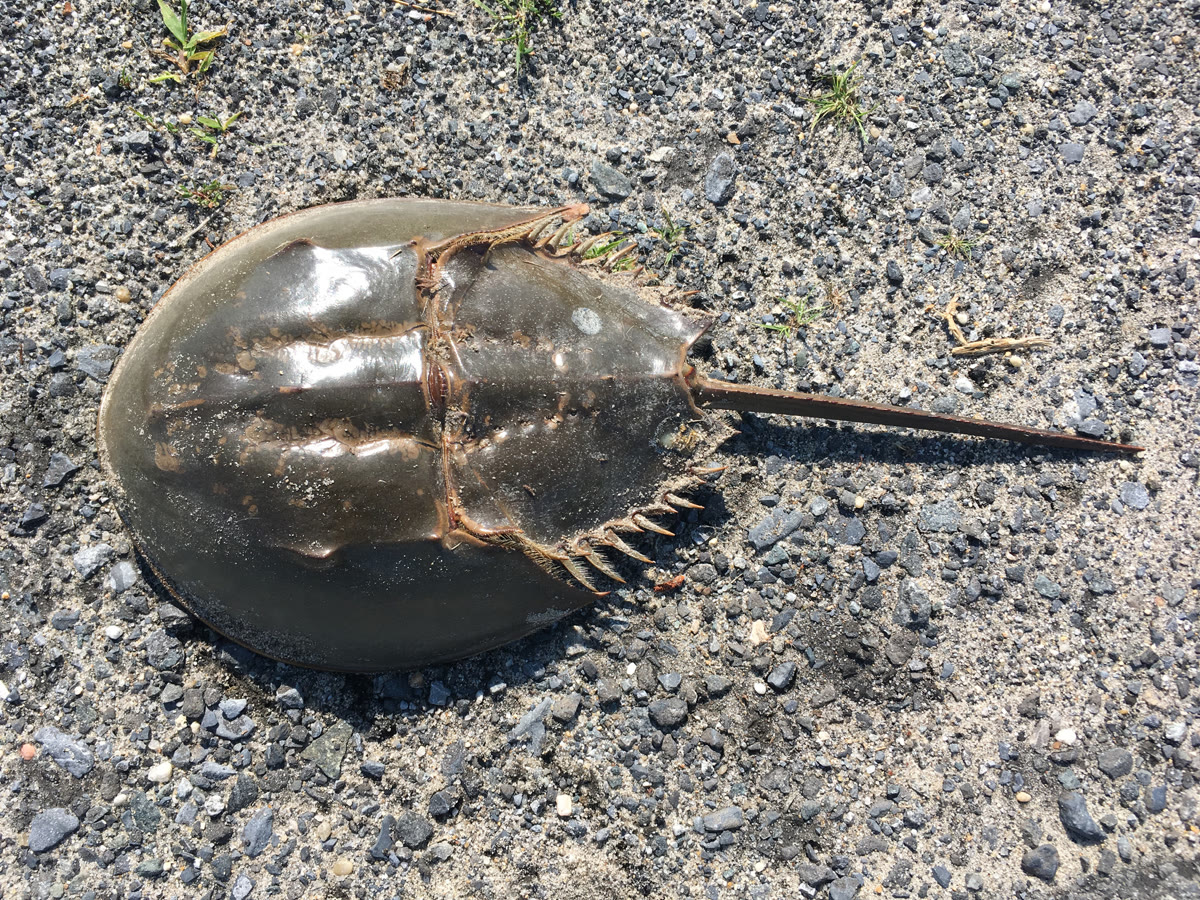
\includegraphics[width=0.5\linewidth]{images/book4/horseshoe-crab.jpg}

{\small An Atlantic horseshoe crab. Its blood carries oxygen on haemocyanin, a
copper protein, and is blue when oxygenated. Photograph: Kaldari, CC0.}
\end{omfigure}

\section{Metals in biology}

\begin{definition}[Metalloproteins]\label{def:b3:bioinorganic:metalloprotein}
A \emph{metalloprotein}\index{metalloprotein} is a protein that contains
bound metal ions; a \emph{metalloenzyme}\index{metalloenzyme} is one that
catalyses a reaction. A \emph{cofactor}\index{cofactor} is a non-protein species,
a metal ion or a small molecule, bound to a protein and needed for its
activity.
\end{definition}

The metals that matter in quantity are sodium, potassium, magnesium and
calcium, which mostly carry charge and hold structures; the transition metals
iron, zinc, copper, manganese, cobalt, molybdenum and nickel occur in traces
but run much of the chemistry. A protein chooses its metal through the donor
atoms it offers and their geometry.

\begin{definition}[Hard and soft acids]\label{def:b3:bioinorganic:hsab}
A \emph{hard acid}\index{hard acid} is a small, highly charged, weakly
polarisable Lewis acid ($\ce{H+}$, $\ce{Mg^2+}$, $\ce{Ca^2+}$, $\ce{Fe^3+}$); a \emph{soft
acid}\index{soft acid} is a large, polarisable one of low charge ($\ce{Cu+}$, $\ce{Ag+}$,
$\ce{Hg^2+}$, $\ce{Cd^2+}$). The \emph{hard and soft acid--base principle}\index{hard and soft acid--base principle}
states that hard acids bind preferably to hard bases
(oxygen donors, fluoride) and soft acids to soft bases (sulfur donors, iodide).
\end{definition}

In proteins, carboxylates and phenolates are hard, the thiolate of cysteine and
the thioether of methionine soft, and the imidazole of histidine in between. Iron(III)
sits among oxygen donors, copper(I) among sulfur donors, zinc, a borderline
acid, with histidine and cysteine; mercury and cadmium are toxic in part
because they seize the cysteines of \omterm{def:b3:complex-kinetics:enzyme}{enzymes}.

\begin{definition}[Irving--Williams series]\label{def:b3:bioinorganic:irving-williams}
The \emph{Irving--Williams series}\index{Irving--Williams series} is the order
of stability of the high-spin complexes of the divalent ions of the first
transition series with a given ligand:
$\ce{Mn^2+} < \ce{Fe^2+} < \ce{Co^2+} < \ce{Ni^2+} < \ce{Cu^2+} > \ce{Zn^2+}$.
\end{definition}

\begin{proposition}[Irving--Williams order]\label{prop:b3:bioinorganic:irving-williams}
The series holds for almost all ligands (an experimental observation); it
follows the decrease of ionic radius from manganese to copper, the ligand-field
stabilisation energy, zero for $d^5$, largest for $d^8$, and the Jahn--Teller
distortion of copper(II), which shortens four of its bonds.
\end{proposition}

\begin{proof}[Argued]
The radius falls across the row as the nuclear charge grows, which strengthens
the electrostatic attraction of every ligand. The ligand-field stabilisation of
high-spin octahedral ions (\cref{ch:b3:complex-spectra-magnetism}) is $0$, $4$,
$8$, $12$ and $6\,\mathrm{Dq}$ for $d^5$ to $d^9$, and $0$ for $d^{10}$: it adds to the trend up to nickel and
drops for zinc; copper(II) recovers more than its stabilisation suggests by
its tetragonal distortion, which gives four short, strong bonds.
\end{proof}

A consequence that cells must manage: copper and zinc would outcompete the
other ions for most sites, so their free concentrations are kept extremely low
by dedicated carrier proteins.

\section{Oxygen transport}

\begin{definition}[Porphyrins and haem]\label{def:b3:bioinorganic:haem}
A \emph{porphyrin}\index{porphyrin} is a large, flat, aromatic macrocycle of four
pyrrole rings joined by methine bridges, whose four nitrogens bind a metal ion
at its centre. \emph{Haem}\index{haem} is the iron complex of protoporphyrin~IX,
the \omterm{def:b3:bioinorganic:metalloprotein}{cofactor} of haemoglobin, myoglobin and the cytochromes.
\end{definition}

In myoglobin and haemoglobin, the iron of \omterm{def:b3:bioinorganic:haem}{haem} has a fifth ligand below the
ring, the nitrogen of the proximal histidine, and a sixth site free for $\ce{O2}$.
Deoxy iron(II) is high spin: an electron in the $d_{x^2-y^2}$ orbital, pointing at the four
nitrogens, makes it too large for the hole of the ring, and it sits out of the
plane, towards the histidine. On binding $\ce{O2}$ it becomes low spin, smaller, and
moves into the plane, pulling the histidine and the protein helix with it.

\begin{omfigure}
% ledger: pdb:Hb.deoxy.FeN4, pdb:Hb.oxy.FeN4
\begin{tikzpicture}[font=\small, scale=0.9]
  \foreach \x/\lab/\dz/\oxy in {0/deoxy (high spin)/-0.34/0, 6.4/oxy (low spin)/-0.04/1} {
    \begin{scope}[xshift=\x cm]
      \draw[omDef, line width=2.6pt] (-2.2,0) -- (2.2,0);
      \node[font=\scriptsize, anchor=west, omDef] at (2.3,0) {porphyrin};
      \fill[omThm] (0,\dz*1.5) circle (0.22);
      \node[font=\scriptsize, anchor=north west] at (0.2,\dz*1.5-0.12) {Fe};
      \draw[black!70, line width=1pt] (0,\dz*1.5-0.22) -- (0,-1.55);
      \node[draw=black!70, regular polygon, regular polygon sides=5, minimum size=7mm, inner sep=0pt] at (0,-1.95) {};
      \node[font=\scriptsize, anchor=west] at (0.45,-1.95) {proximal His};
      \node[font=\small\bfseries] at (0,1.9) {\lab};
      \ifnum\oxy=1
        \draw[black!70, line width=1pt] (0,0.2) -- (0,0.85) -- (0.55,1.25);
        \fill[red!75] (0,0.85) circle (0.13) (0.55,1.25) circle (0.13);
        \node[font=\scriptsize, anchor=west] at (0.75,1.2) {$\ce{O2}$, bent};
      \fi
    \end{scope}
  }
  \draw[<->, black!60] (-1.0,0) -- (-1.0,-0.51) node[midway, left, font=\scriptsize] {\qty{0.34}{\angstrom}};
\end{tikzpicture}

{\small The \omterm{def:b3:bioinorganic:haem}{haem} iron seen edge-on, its displacement from the ring drawn to
scale (1~\AA{} as 1.35~cm; the other distances are schematic). In deoxyhaemoglobin the high-spin iron(II) lies
\qty{0.34}{\angstrom} below the mean plane of the four pyrrole nitrogens, on the side of the
proximal histidine; in oxyhaemoglobin it is within \qty{0.05}{\angstrom} of the plane, with $\ce{O2}$
bound end-on and bent (distances computed from crystal structures).}
\end{omfigure}

Bound dioxygen is better described as superoxide on iron(III), $\ce{Fe^{III}-O2^-}$, than as
neutral $\ce{O2}$ on iron(II): the complex is diamagnetic because the unpaired
electrons of the two centres couple. The protein stops the irreversible
oxidation to iron(III) and water, which a bare \omterm{def:b3:bioinorganic:haem}{haem} in water undergoes at
once.

\begin{definition}[Cooperative binding]\label{def:b3:bioinorganic:cooperativity}
Binding to a protein with several sites is \emph{cooperative}\index{cooperative binding}
when the binding of one ligand raises the affinity of the remaining
sites. The \emph{Hill coefficient}\index{Hill coefficient} $n$ is the slope of the
Hill plot, $\log\frac{\theta}{1 - \theta}$ against $\log p$, at half saturation ($\theta$ is the fraction of sites
occupied).
\end{definition}

\begin{proposition}[One site]\label{prop:b3:bioinorganic:hyperbola}
For a protein with one site, $\mathrm{P + O_2 \rightleftharpoons PO_2}$, the fraction occupied is $\theta = p/(p_{50} + p)$, where $p_{50}$ is
the dissociation constant expressed as a pressure.
\end{proposition}

\begin{proof}
$K_d = [\mathrm P]p/[\mathrm{PO_2}] = p_{50}$, so $[\mathrm{PO_2}] = [\mathrm P]p/p_{50}$, and $\theta = [\mathrm{PO_2}]/([\mathrm P] + [\mathrm{PO_2}]) = (p/p_{50})/(1 + p/p_{50})$.
\end{proof}

\begin{theorem}[Hill equation]\label{thm:b3:bioinorganic:hill}
For a protein with $n$ sites that are either all empty or all filled,
$\mathrm{P + n\,O_2 \rightleftharpoons P(O_2)_n}$,
\[
  \theta = \frac{p^n}{p_{50}^n + p^n}, \qquad \log\frac{\theta}{1 - \theta} = n\log p - n\log p_{50}.
\]
\end{theorem}

\begin{proof}
$K_d = [\mathrm P]p^n/[\mathrm{P(O_2)_n}]$; write $K_d = p_{50}^n$. The fraction of sites occupied is that of molecules
in the filled form, $\theta = [\mathrm{P(O_2)_n}]/([\mathrm P] + [\mathrm{P(O_2)_n}]) = (p/p_{50})^n/(1 + (p/p_{50})^n)$. Then $\theta/(1 - \theta) = (p/p_{50})^n$, and taking
logarithms gives the straight line of slope $n$.
\end{proof}

Haemoglobin, with four sites, is not fully \omterm{def:b3:bioinorganic:cooperativity}{cooperative}: its \omterm{def:b3:bioinorganic:cooperativity}{Hill coefficient} is
well below 4, about 3, and its Hill plot has slope 1 at both ends, where
it behaves as a deoxy or as an oxy protein with independent sites. The
cooperativity comes from a change of quaternary structure: the motion of the
iron into the plane of the first \omterm{def:b3:bioinorganic:haem}{haem} to bind $\ce{O2}$ is passed to the other subunits.

\begin{omfigure}
\begin{tikzpicture}
\begin{axis}[name=a, width=0.48\linewidth, height=5.6cm, xmin=0, xmax=14, ymin=0, ymax=1.02,
  axis lines=left, xlabel={$p(\ce{O2})$ / \unit{kPa}}, ylabel={saturation $\theta$},
  tick label style={font=\scriptsize}, label style={font=\small}]
\addplot[omMeth, thick] table[x=p, y=Mb] {figdata/out/bachelor-3-oxygen-binding.dat};
\addplot[omThm, thick] table[x=p, y=Hb] {figdata/out/bachelor-3-oxygen-binding.dat};
\addplot[omThm, thick, dashed] table[x=p, y=Hbacid] {figdata/out/bachelor-3-oxygen-binding.dat};
\draw[black!35] (axis cs:5,0) -- (axis cs:5,1.0) (axis cs:13,0) -- (axis cs:13,1.0);
\node[font=\scriptsize, anchor=south] at (axis cs:5,0.02) {tissues};
\node[font=\scriptsize, anchor=south east] at (axis cs:13,0.02) {lungs};
\node[font=\scriptsize, omMeth] at (axis cs:1.9,0.96) {Mb};
\node[font=\scriptsize, omThm] at (axis cs:7.5,0.6) {Hb};
\end{axis}
\begin{axis}[at={(a.east)}, anchor=west, xshift=1.4cm, width=0.48\linewidth, height=5.6cm,
  xmin=-1.5, xmax=1.5, ymin=-3, ymax=3, axis lines=left,
  xlabel={$\log_{10}(p/\unit{kPa})$}, ylabel={$\log_{10}\bigl(\theta/(1-\theta)\bigr)$},
  tick label style={font=\scriptsize}, label style={font=\small}]
\draw[black!30] (axis cs:-1.5,0) -- (axis cs:1.5,0);
\addplot[omMeth, thick] table[x=lgp, y=Mb] {figdata/out/bachelor-3-oxygen-binding-b.dat};
\addplot[omThm, thick, restrict y to domain=-3:3] table[x=lgp, y=Hb] {figdata/out/bachelor-3-oxygen-binding-b.dat};
\node[font=\scriptsize, omMeth, anchor=west] at (axis cs:-1.1,1.4) {slope 1};
\node[font=\scriptsize, omThm, anchor=west] at (axis cs:0.75,-1.5) {slope 2.7};
\end{axis}
\end{tikzpicture}

{\small Left: oxygen saturation of myoglobin (green) and haemoglobin (red;
dashed: at a lower pH) against the pressure of oxygen, with model values
$p_{50} = \qty{0.37}{kPa}$ (Mb) and \qty{3.5}{kPa} (Hb), $n = 2.7$. Between the lungs and the tissues haemoglobin
gives up a quarter of its oxygen, myoglobin almost none. Right: the
corresponding Hill plots, straight lines in this model (real haemoglobin's plot
bends to slope 1 at both ends).}
\end{omfigure}

\begin{method}[Reading a Hill plot]\label{met:b3:bioinorganic:hill-plot}
\begin{enumerate}
  \item From each measured saturation compute $\log(\theta/(1 - \theta))$; plot it against $\log p$.
  \item The pressure where the plot crosses zero is $p_{50}$.
  \item The slope at that point is the \omterm{def:b3:bioinorganic:cooperativity}{Hill coefficient}: $n = 1$ means independent
        sites, $n > 1$ \omterm{def:b3:bioinorganic:cooperativity}{cooperative binding}.
  \item With two points only, $n = \Delta\log(\theta/(1 - \theta))/\Delta\log p$.
\end{enumerate}
\end{method}

Haemoglobin also binds protons and carbon dioxide at sites away from the \omterm{def:b3:bioinorganic:haem}{haem},
which shift its curve to the right where they are abundant, in working tissues:
the Bohr effect releases more oxygen exactly where it is needed.

\begin{proposition}[Carbon monoxide competition]\label{prop:b3:bioinorganic:haldane}
If carbon monoxide and dioxygen compete for the same sites, with
$\mathrm{HbO_2 + CO \rightleftharpoons HbCO + O_2}$ of equilibrium constant $M$, then
$[\mathrm{HbCO}]/[\mathrm{HbO_2}] = M\,p(\ce{CO})/p(\ce{O2})$.
\end{proposition}

\begin{proof}
At equilibrium $M = [\mathrm{HbCO}]\,p(\ce{O2})/([\mathrm{HbO_2}]\,p(\ce{CO}))$; rearranging gives the result.
\end{proof}

$M$ is in the hundreds for human haemoglobin, so that a few hundred parts per
million of carbon monoxide occupy a large fraction of the sites; worse, the
sites left free hold their oxygen more tightly, as the cooperativity
works on them. Free \omterm{def:b3:bioinorganic:haem}{haem} binds carbon monoxide far more strongly still: in
the protein, a distal histidine above the iron hinders the linear Fe--C--O
geometry carbon monoxide prefers, while it hydrogen-bonds the bent $\ce{O2}$.
Other animals use other metals: the haemocyanins of molluscs and arthropods
bind $\ce{O2}$ between two copper ions as peroxide, the haemerythrins of some marine
worms on a pair of iron ions.

\begin{inthelab}[An oxygen-binding curve]
A solution of haemoglobin in buffer is placed in a gas-tight cuvette fitted
with a side flask. It is first freed of oxygen by flushing with nitrogen, then
known volumes of air are injected and the solution equilibrated by gentle
tilting. After each addition the visible spectrum is recorded: the bands of
the deoxy form (one band near \qty{555}{nm}) give way to the two bands of the oxy form,
and the saturation is read from the absorbance at one wavelength, between its
deoxy and oxy limits.
\end{inthelab}

\section{Metalloenzymes}

Carbonic anhydrase speeds up $\ce{CO2 + H2O <=> HCO3- + H+}$, which in water alone takes
seconds, enough to matter in the red cell's short passage through a lung
capillary. Its zinc ion is held by three histidines and a water molecule. A
small cation of high charge, it lowers the $\mathrm pK_a$ of that water from about 14 to
about 7: at physiological pH a good part of the \omterm{def:b3:complex-kinetics:enzyme}{enzyme} carries a zinc-bound
hydroxide, a strong nucleophile, held right next to a pocket that binds $\ce{CO2}$.

\begin{omfigure}
\begin{tikzpicture}[font=\small, >=Stealth]
  \node (a) at (90:2.0) {$\mathrm{(His)_3Zn{-}OH_2}$};
  \node (b) at (0:2.9) {$\mathrm{(His)_3Zn{-}OH^-}$};
  \node (c) at (-90:2.0) {$\mathrm{(His)_3Zn{-}OCO_2H^-}$};
  \draw[->, thick] (a) to[bend left=25] node[midway, above right, font=\scriptsize] {$-\,\ce{H+}$ (to a histidine shuttle)} (b);
  \draw[->, thick] (b) to[bend left=25] node[midway, below right, font=\scriptsize, align=left] {$+\,\ce{CO2}$:\\ nucleophilic attack} (c);
  \draw[->, thick] (c) to[bend left=35] node[midway, left, font=\scriptsize, align=right] {$+\,\ce{H2O}$\\ $-\,\ce{HCO3-}$} (a);
\end{tikzpicture}

{\small The catalytic cycle of carbonic anhydrase. The zinc-bound water loses a
proton; the zinc-bound hydroxide attacks carbon dioxide; water displaces the
hydrogencarbonate. The proton transfer to the solvent is the slowest step.}
\end{omfigure}

\begin{proposition}[A fast enzyme]\label{prop:b3:bioinorganic:carbonic-anhydrase}
The \omterm{def:b3:complex-kinetics:michaelis}{specificity constant} $k_{\mathrm{cat}}/K_M$ of carbonic anhydrase approaches the rate
constant of encounter of $\ce{CO2}$ with the \omterm{def:b3:complex-kinetics:enzyme}{enzyme}: nearly every encounter leads to
reaction.
\end{proposition}

\begin{proof}[Argued]
$k_{\mathrm{cat}}/K_M$ is the second-order rate constant of \omterm{def:b3:complex-kinetics:enzyme}{enzyme} and substrate at low substrate
concentration (\cref{ch:b3:complex-kinetics}); it cannot exceed the
\omterm{def:b3:rate-theories:diffusion}{diffusion-controlled} rate constant of their encounter
(\cref{ch:b3:rate-theories}). The measured values for carbonic anhydrase are
among the highest known for any \omterm{def:b3:complex-kinetics:enzyme}{enzyme} and approach that limit: the chemistry
inside the \omterm{def:b3:complex-kinetics:enzyme}{active site} is then no longer what limits the rate.
\end{proof}

Cytochrome P450 \omterm{def:b3:complex-kinetics:enzyme}{enzymes}, in the liver and in many other cells, hydroxylate C--H
bonds of drugs and hormones. Their \omterm{def:b3:bioinorganic:haem}{haem} iron is held by a cysteine thiolate; with
$\ce{O2}$ and two electrons it forms an iron(IV)-oxo complex with a radical on the
\omterm{def:b3:bioinorganic:haem}{porphyrin}, called compound I, which abstracts a hydrogen atom from the
substrate and returns the hydroxyl group to the carbon radical. Nitrogenase
reduces $\ce{N2}$ to ammonia at room temperature on a cluster of seven iron atoms,
one molybdenum and nine sulfides around a central carbon atom, the FeMo
\omterm{def:b3:bioinorganic:metalloprotein}{cofactor}, at the cost of many molecules of ATP. Vitamin $\mathrm{B_{12}}$ contains a
cobalt--carbon bond, one of the very few metal--carbon bonds in biology, whose
homolysis starts radical rearrangements.

\section{Electron transfer and energy}

Proteins that only move electrons have metal centres with small
reorganisation energies (\cref{ch:b3:complex-mechanisms}): the two oxidation
states have almost the same geometry, so that the Marcus barrier is low.

\begin{definition}[Iron--sulfur clusters]\label{def:b3:bioinorganic:fes}
An \emph{iron--sulfur cluster}\index{iron--sulfur cluster} is a group of iron
ions bridged by sulfide ions and bound to the protein by cysteine thiolates:
$\ce{[2Fe-2S]}$, $\ce{[3Fe-4S]}$ and the cubane-like $\ce{[4Fe-4S]}$.
\end{definition}

\begin{definition}[Blue copper proteins]\label{def:b3:bioinorganic:blue-copper}
A \emph{blue copper protein}\index{blue copper protein} carries one copper
ion bound by two histidines, a cysteine and a weakly bound methionine in a
distorted tetrahedral site; its intense blue colour comes from a
cysteine-to-copper(II) charge-transfer band.
\end{definition}

\begin{definition}[Entatic state]\label{def:b3:bioinorganic:entatic}
The \emph{entatic state}\index{entatic state} is a metal site held by the
protein in a strained geometry, between the geometries preferred by its two
oxidation states, which lowers the \omterm{def:b3:complex-mechanisms:reorganisation}{reorganisation energy} of its reactions.
\end{definition}

Copper(II) alone prefers a square plane, copper(I) a tetrahedron: in the blue
copper site neither is satisfied, and electron transfer is fast.

\begin{definition}[Oxygen-evolving complex]\label{def:b3:bioinorganic:oec}
The \emph{oxygen-evolving complex}\index{oxygen-evolving complex} of
photosystem~II is the $\mathrm{Mn_4CaO_5}$ cluster that oxidises water to dioxygen in
photosynthesis.
\end{definition}

\begin{proposition}[Four photons per oxygen]\label{prop:b3:bioinorganic:kok}
Oxidising two water molecules to one $\ce{O2}$ requires four photons absorbed by
photosystem~II, the cluster passing through five states $\mathrm S_0$ to $\mathrm S_4$.
\end{proposition}

\begin{proof}
$\ce{2H2O -> O2 + 4H+ + 4e-}$: four electrons must be removed. Each photon absorbed by the
reaction centre moves one electron away from it, and the cluster refills the
oxidised centre one electron at a time: four photons, four steps, storing
oxidising equivalents in the states $\mathrm S_1$ to $\mathrm S_4$; $\mathrm S_4$ releases $\ce{O2}$ and returns to $\mathrm S_0$.
\end{proof}

\begin{omfigure}
\begin{tikzpicture}[font=\small, >=Stealth]
  \foreach \i/\ang in {0/90, 1/18, 2/-54, 3/-126, 4/162} {
    \node[draw, circle, minimum size=9mm, fill=omDef!10] (s\i) at (\ang:2.0) {$\mathrm S_{\i}$};
  }
  \foreach \i/\j in {0/1, 1/2, 2/3, 3/4} {
    \draw[->, thick] (s\i) to[bend left=18] node[midway, sloped, above, font=\scriptsize] {$h\nu$, $-\mathrm e^-$} (s\j);
  }
  \draw[->, thick, omThm] (s4) to[bend left=18] node[midway, sloped, above, font=\scriptsize] {$-\ce{O2}$, $+\,\ce{2H2O}$} (s0);
\end{tikzpicture}

{\small The Kok cycle of the \omterm{def:b3:bioinorganic:oec}{oxygen-evolving complex}. Each photon absorbed by
photosystem~II removes one electron from the manganese cluster (protons
leave on the way); the fourth oxidation gives $\mathrm S_4$, which releases dioxygen and
binds two water molecules again.}
\end{omfigure}

At the other end of the energy chain, cytochrome $c$ oxidase of the
mitochondria reduces $\ce{O2}$ to water with four electrons and four protons on a
\omterm{def:b3:bioinorganic:haem}{haem} iron and a copper ion facing each other, without releasing the partly
reduced, damaging superoxide or peroxide.

\section{Metals in medicine}

\begin{definition}[Metallodrugs]\label{def:b3:bioinorganic:metallodrug}
A \emph{metallodrug}\index{metallodrug} is a drug whose activity depends on a
metal ion or a metal complex.
\end{definition}

Cisplatin, \textit{cis}-$\ce{[PtCl2(NH3)2]}$, is stable in blood, where the chloride concentration is
high; inside cells, where it is much lower, it exchanges a chloride for water
(\cref{ch:b3:complex-mechanisms}). The aqua complex binds the N7 atom of
guanine, then a second guanine next to it on the same strand: the 1,2-GG
cross-link bends the DNA, which the cell cannot repair, and it dies. The
\textit{trans} isomer cannot bridge two neighbouring bases and is inactive.
Carboplatin, with a chelating dicarboxylate that leaves slowly, has fewer
side effects; oxaliplatin, with a diaminocyclohexane ligand, works on tumours
resistant to cisplatin.

\begin{omfigure}
\begin{tikzpicture}[font=\small]
  \draw[black!60, line width=1.4pt] (-3.2,0) -- (3.2,0);
  \node[font=\scriptsize, anchor=west] at (3.3,0) {DNA strand};
  \foreach \x/\b in {-2.4/C, -1.0/G, 1.0/G, 2.4/T} {
    \draw[black!60, line width=1pt] (\x,0) -- (\x,0.6);
    \node[draw=black!70, fill=white, rounded corners=1pt, minimum width=6mm] (n\b\x) at (\x,0.9) {\b};
  }
  \node (pt) at (0,2.4) {$\ce{Pt}$};
  \draw[omThm, thick] (pt) -- (-0.95,1.2) node[midway, left, font=\scriptsize] {N7};
  \draw[omThm, thick] (pt) -- (0.95,1.2) node[midway, right, font=\scriptsize] {N7};
  \draw (pt) -- (-0.5,3.1) node[above left, font=\scriptsize, inner sep=1pt] {$\ce{H3N}$};
  \draw (pt) -- (0.5,3.1) node[above right, font=\scriptsize, inner sep=1pt] {$\ce{NH3}$};
\end{tikzpicture}

{\small The 1,2-intrastrand cross-link made by cisplatin, schematic: after
losing its two chlorides, platinum binds the N7 atoms of two adjacent guanines
of one strand, keeping its two \textit{cis} ammine ligands. The real adduct
bends the double helix.}
\end{omfigure}

\begin{definition}[Contrast agents]\label{def:b3:bioinorganic:contrast}
A \emph{contrast agent}\index{contrast agent} for magnetic resonance imaging is
a paramagnetic compound that shortens the relaxation times of nearby water
protons. Its \emph{relaxivity}\index{relaxivity} $r_1$ is the increase of the
relaxation rate $1/T_1$ per unit concentration of the agent.
\end{definition}

\begin{proposition}[Relaxation rate]\label{prop:b3:bioinorganic:relaxivity}
With an agent of \omterm{def:b3:bioinorganic:contrast}{relaxivity} $r_1$ at concentration $c$, the relaxation rate of water
protons is $1/T_1 = 1/T_{1,0} + r_1c$, where $T_{1,0}$ is the value without agent.
\end{proposition}

\begin{proof}
The paramagnetic contribution is proportional to the number of agent molecules
that water molecules visit per unit time, hence to $c$; relaxation rates from
independent mechanisms add. By definition of $r_1$ the added rate is $r_1c$.
\end{proof}

Gadolinium(III), $4f^7$ with seven unpaired electrons and a slowly relaxing
electron spin, is the metal of choice. Free $\ce{Gd^3+}$ is toxic: it is given as a
very stable complex of an octadentate polyaminocarboxylate that leaves one
site for a water molecule, which exchanges fast with the bulk and carries the
relaxation to all of it.

\begin{definition}[Chelation therapy]\label{def:b3:bioinorganic:chelation-therapy}
\emph{Chelation therapy}\index{chelation therapy} is the removal of a toxic
metal from the body by a chelating ligand given as a drug, which forms a stable,
soluble complex that is excreted.
\end{definition}

\begin{method}[Choosing a chelating drug]\label{met:b3:bioinorganic:choose-chelator}
\begin{enumerate}
  \item Compare the stability constants of the chelator with the toxic metal
        and with the essential metals present in large amounts ($\ce{Ca^2+}$, $\ce{Mg^2+}$,
        $\ce{Zn^2+}$).
  \item Compute the free metal level $\mathrm{pM} = -\log[\mathrm M]$ the chelator leaves at the
        concentrations and pH of the body: the higher pM for the toxic metal and the
        lower for the essential ones, the better.
  \item Give the chelator already loaded with the competing essential ion (the
        calcium complex of EDTA for lead), so that it exchanges rather than
        strips calcium from the blood.
  \item Check the hard--soft match (sulfur donors for mercury and lead, hard
        oxygen donors for iron(III)) and that the complex is excreted.
\end{enumerate}
\end{method}

\begin{safety}{\ghs[0.62cm]{GHS05}\ghs[0.62cm]{GHS06}\ghs[0.62cm]{GHS08}}
% ledger: ghs4:cisplatin
Cisplatin: fatal if swallowed, may cause cancer and genetic defects, may damage
fertility, causes serious eye damage and allergic reactions; it is handled
only as a prepared drug solution, with gloves, in a ventilated cabinet.
\end{safety}

\begin{history}[A protein structure and an accidental drug]
Max Perutz worked for more than twenty years on the X-ray structure of
haemoglobin, solved at low resolution in 1959; with John Kendrew, who solved
myoglobin, he received the 1962 Nobel Prize in Chemistry. In 1965 Barnett
Rosenberg, passing a current between platinum electrodes in a culture of
bacteria, saw them grow into long filaments without dividing; the cause was
not the current but a platinum ammine complex formed from the electrodes. It
became cisplatin, still one of the most used anticancer drugs.
\end{history}

\section{Exercises}

\begin{exercise}[$\star$]\label{exo:b3:bioinorganic:1}
A protein is 20\,\% saturated at \qty{2.1}{kPa} of oxygen and 80\,\% at \qty{5.9}{kPa}. Compute its
\omterm{def:b3:bioinorganic:cooperativity}{Hill coefficient}.
\end{exercise}

\begin{exercise}[$\star$]\label{exo:b3:bioinorganic:2}
Order $\ce{Zn^2+}$, $\ce{Mn^2+}$, $\ce{Cu^2+}$, $\ce{Fe^2+}$, $\ce{Ni^2+}$ and $\ce{Co^2+}$ by the stability of their complexes with
a given ligand, and explain the place of zinc.
\end{exercise}

\begin{exercise}[$\star$]\label{exo:b3:bioinorganic:3}
Predict the preferred protein donors (carboxylate, cysteine thiolate,
histidine imidazole) of $\ce{Ca^2+}$, $\ce{Fe^3+}$, $\ce{Cu+}$, $\ce{Zn^2+}$ and $\ce{Hg^2+}$.
\end{exercise}

\begin{exercise}[$\star$]\label{exo:b3:bioinorganic:4}
How many electrons are removed, and how many photons absorbed by photosystem~II,
per molecule of $\ce{O2}$ evolved? Per mole?
\end{exercise}

\begin{exercise}[$\star\star$]\label{exo:b3:bioinorganic:5}
With the model curves of the chapter ($p_{50} = \qty{0.37}{kPa}$ for myoglobin; \qty{3.5}{kPa} and $n = 2.7$ for
haemoglobin), compute the fraction of its oxygen each protein gives up between
\qty{13}{kPa} (lungs) and \qty{5}{kPa} (tissues).
\end{exercise}

\begin{exercise}[$\star\star$]\label{exo:b3:bioinorganic:6}
Air containing \qty{50}{ppm} of carbon monoxide is breathed for long enough to reach
equilibrium. With $M = 230$ (data of the exercise) and $p(\ce{O2})/p(\ce{CO})$ that of the air
(20.95\,\% oxygen), what fraction of the haemoglobin carries CO?
\end{exercise}

\begin{exercise}[$\star\star$]\label{exo:b3:bioinorganic:7}
Give the formal oxidation states of the iron ions in the clusters $\ce{[Fe2S2(SR)4]^2-}$,
$\ce{[Fe2S2(SR)4]^3-}$ and $\ce{[Fe4S4(SR)4]^2-}$ (SR: cysteinate, S: sulfide).
\end{exercise}

\begin{exercise}[$\star\star$]\label{exo:b3:bioinorganic:8}
Write the first aquation of cisplatin, and explain why it is slow in blood and
faster inside cells. Which atom of DNA does platinum bind, and why is the
\textit{trans} isomer inactive?
\end{exercise}

\begin{exercise}[$\star\star$]\label{exo:b3:bioinorganic:9}
A tissue has $T_1 = \qty{1.2}{s}$. A gadolinium agent of \omterm{def:b3:bioinorganic:contrast}{relaxivity} $\qty{4.0}{L.mmol^{-1}.s^{-1}}$ reaches \qty{0.10}{mmol/L}
in it (data of the exercise). Compute the new $T_1$.
\end{exercise}

\begin{exercise}[$\star\star\star$]\label{exo:b3:bioinorganic:10}
A chelator L has $\log K = 18.0$ with $\ce{Pb^2+}$ and $10.7$ with $\ce{Ca^2+}$ (data of the exercise).
Compute the equilibrium constant of $\ce{Pb^2+ + [CaL]^2- <=> [PbL]^2- + Ca^2+}$ and explain why the calcium
complex is given rather than the free ligand.
\end{exercise}

\begin{exercise}[$\star\star\star$]\label{exo:b3:bioinorganic:11}
% ledger: enz:median.kcatKM
Carbonic anhydrase has $k_{\mathrm{cat}}/K_M \approx \qty{1e8}{L.mol^{-1}.s^{-1}}$ (data of the exercise), a typical \omterm{def:b3:complex-kinetics:enzyme}{enzyme} about
$\qty{1e5}{L.mol^{-1}.s^{-1}}$. At $[\ce{CO2}] = \qty{1.0}{mmol/L}$, far below $K_M$, compare the time each needs to convert half
the substrate with an \omterm{def:b3:complex-kinetics:enzyme}{enzyme} concentration of \qty{1.0}{\micro mol/L}.
\end{exercise}

\begin{exercise}[$\star\star\star$]\label{exo:b3:bioinorganic:12}
With $M = 230$, what pressure of carbon monoxide occupies half the sites in the
presence of air at \qty{0.2095}{bar} of oxygen? Express it in ppm of a gas at \qty{1}{bar}.
\end{exercise}

\section{Problem: How Much Oxygen Does Blood Deliver?}

\begin{problem}[{Weekend problem --- how much oxygen does blood deliver? Hill
curves of haemoglobin and myoglobin, the oxygen carried by a litre of blood, the
Bohr shift, and what carbon monoxide takes away}]
\label{pb:b3:bioinorganic:1}
% ledger: const:Vm1
Model data of the problem: haemoglobin $p_{50} = \qty{3.5}{kPa}$ and $n = 2.7$ at pH 7.4, $p_{50} = \qty{4.0}{kPa}$ at the
lower pH of working tissues; myoglobin $p_{50} = \qty{0.37}{kPa}$; blood contains \qty{150}{g/L} of
haemoglobin, of molar mass \qty{64.5}{kg/mol}, with four sites per molecule; $p(\ce{O2})$ is \qty{13}{kPa}
in the lungs and \qty{5.0}{kPa} in the tissues; the heart pumps \qty{5.0}{L/min} at rest;
$M = 230$ for carbon monoxide. Gas volumes at \qty{273.15}{K} and \qty{101.325}{kPa}.

\medskip\noindent\textbf{Part I --- The curves.}
\begin{enumerate}
  \item Compute the saturation of haemoglobin in the lungs.
  \item Compute it in the tissues at pH 7.4.
  \item Compute the saturation of myoglobin at \qty{5.0}{kPa}.
  \item Why can myoglobin take oxygen from haemoglobin in a muscle?
  \item What \omterm{def:b3:bioinorganic:cooperativity}{Hill coefficient} would four independent sites give?
  \item Explain in one sentence where the cooperativity comes from.
\end{enumerate}

\medskip\noindent\textbf{Part II --- A litre of blood.}
\begin{enumerate}[resume]
  \item Compute the concentration of haemoglobin in mol/L.
  \item Compute the concentration of oxygen sites.
  \item Compute the oxygen carried per litre in the lungs, in mmol.
  \item Compute the oxygen delivered per litre to the tissues at pH 7.4.
  \item Convert it to millilitres of gas.
  \item What fraction of the oxygen carried is that?
\end{enumerate}

\medskip\noindent\textbf{Part III --- The Bohr shift.}
\begin{enumerate}[resume]
  \item Compute the saturation in the tissues at the lower pH.
  \item Compute the oxygen delivered per litre with the shift.
  \item By what factor does the shift increase delivery?
  \item What lowers the pH of a working muscle?
  \item Compute the oxygen delivered per minute at rest, in mmol.
  \item Convert it to litres of gas per minute.
\end{enumerate}

\medskip\noindent\textbf{Part IV --- Carbon monoxide.}
\begin{enumerate}[resume]
  \item Compute $[\mathrm{HbCO}]/[\mathrm{HbO_2}]$ for air with \qty{100}{ppm} of CO.
  \item Compute the fraction of sites lost to CO.
  \item Why is the loss of delivered oxygen worse than that fraction?
  \item Why is pure oxygen the first treatment?
  \item Why does the distal histidine matter for survival?
  \item State the result: the litres of oxygen delivered per minute at rest.
\end{enumerate}
\end{problem}
